\documentclass{article}
\usepackage[utf8]{inputenc}
\usepackage[T1]{fontenc}


\usepackage{graphicx}
\graphicspath{ {images/} }
\title{Fast vertex cover with double star graphs}
\date{2018\\ May}
\author{Samuel Chase\\ Based on \textit{Covering by trees of small diameter} by Lov\'asz}
\begin{document}
	\maketitle
	\section{Introduction}
	In his paper \textit{Covering by trees of small diameter}, Lov\'asz discusses double star trees. Double star trees are trees of diameter less than or equal to 3. A double star can be formed by taking any two star graphs, and drawing an edge between the central nodes of the star, as seen in Figure 1
	\begin{figure}[h]
		\caption{}
		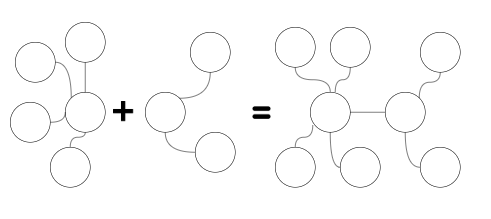
\includegraphics{Figure1}
	\end{figure}
	
	Double stars also have the interesting property of being able to cover grap hs incredibly quickly. In fact, a graph of n vertices be covered by a greedy algorithm taking at most $2n/3$ steps. All that is required to cover a graph with double stars is to find a maximal matching of edges, and then draw double stars centered around those edges,where the two vertices connected to the edge form the individual single stars. Lov\'asz has proved this to be true, and that $2n/3$ double stars are required. Discussed in this paper will be the key determinants in a maximal double-star cover, as well as examples of such covers on simple graphs.
	\section{The algorithm}
	
	Lov\'asz begins by asserting that $\tau$ is the maximum number of independent vertices of $G$. He also states that $M$ as the maximal matching of $G$, having size $r$. $I$ is defined as the vertices not covered by $M$, with a size of $s$. If $n$ = $2r$ then $I$ = $\emptyset$.
	\\\\
	In section 2 it is stated that $f_{3}(g)$ is the maximum number of double stars required to cover a graph. We also know $f_{3}(g) \leq f_{2}(g)$ as in the worst case it is still impossible that double stars cover worse than single stars. This leads Lov\'as to know that $n-\tau \leq n-s = 2r$, or the number of vertices minus independent vertices is less than or rqual to the vertices minus the vertices consained in $I$, which is equal to the number of vertices in $M$.
	\\\\
	In section 3 Lov\'asz moves on to looking at $S_{i}$. $S_{i}$ is a double star of parts of $M$. $T_{i}$ is the tree of all edges containing $c_{i}$ (from $i$). We know that the set of all $S$ and $T$ covers $G$, therefore $f_{3}(g) \leq r + s = n - r$, or the maximum number of double stars required to cover a graphis less than or equal to the size of $m$ plus the size of $i$, which is equal to the size of $g$ minus the size of $m$.
	\\\\
	Combining what is learned in section 4 we are able to prove Lov\'asz's theorem, that $f_{3}(g) \leq 2n/3$
	
		\section{Examples}
		Presented below are examples of graphs of various sizes. It may be noted that some of these graphs themselves are double stars. This reveals some of the inefficiency with this algorithm - even when a small cover (potentially even one of size 1) is available a larger cover may be selected simply because of the nature of the greedy algorithm. Similarly, the steps taken will be laid out sequentially, and if different edges are selected the end cover might be very different.
		 \\
				\begin{figure}[h]
				\caption{}
				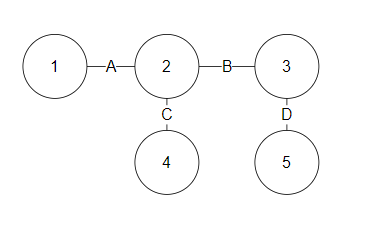
\includegraphics{Figure2}
			\end{figure}
		\\
			Above, in figure 2, we see a double star graph. We know that $n$ is equal to 5. Running our greedy algorithm to find a maximal matching, we will assume we select edges c and d. This means $M = \{c,d\}$, and therefore $r = 2$. $I$ will be all vertices not touched by $M$, therefore $I = \{1\}$ and $s$ = 1. Knowing that $f_{3}(g) \leq n-r$, we can say that the maximum number of double stars necessary to cover this graph is 3. An example of this maximum cover is a cover containing double stars centered around a,b, and c. Assuming we make the odd choice of selecting $a$ and $c$ to be the centers of our first two double stars, we notice that if we add either $b$ or $d$ we will necessarily have a full cover. Although this is something our algorithm would never provide as a cover (due to $a$ and $b$ being adjacent) this shows a theoretical maximum size for the vertex cover. It is simply impossible to increase this value, knowing that no matter which edges we choose in any order we will cover the graph in at most 3 double stars.
	
\end{document}